\documentclass[11pt]{article}
\usepackage[margin=1in]{geometry}
\usepackage{amsmath, amssymb}
\usepackage{booktabs}
\usepackage{graphicx}
\usepackage{float}
\usepackage{hyperref}

\newcommand{\inff}{\mathrm{inf}}
\newcommand{\pers}{\mathrm{pers}}
\newcommand{\surp}{\mathrm{surp}}
\newcommand{\sus}{\mathrm{sus}}
\newcommand{\Sus}{\mathrm{Sus}}
\newcommand{\KL}{\mathrm{KL}}

\title{Three Surprise-Based Detection Scores: Empirical Comparison}
\author{Draft}
\date{2026-04-17}

\begin{document}
\maketitle

\section{Setup}

We compare three per-round scores for detecting a non-informative speaker:
$\surp_2$ (prior predictive surprisal), $\surp_1$ (posterior predictive
surprisal), and $\sus$ (observation-level suspicion).  All three are
computed from the perspective of a credulous $L_1^\inff$ listener; full
definitions and the key algebraic identity
\[
\sus(u) = \surp_2(u)
          - \KL\!\bigl(L_1(\cdot\mid u)\,\|\,L_1(\cdot)\bigr)
          + \Delta H(u)
\]
are given in \texttt{three\_scores.pdf}.  Each score enters the same
sequential test
\[
\Sus(t) > c\cdot \bar\sigma(t)/\sqrt{t},\qquad c = 2.
\]

Parameters: $n=1$ patient, $m=7$ sessions, rationality
$\alpha=3$, $\theta$-space $\{0, 0.1, 0.2, 0.3, 0.4, 0.5, 0.6, 0.7, 0.8, 0.9, 1\}$, $\psi$-space
$\{\inff,\pers^{+},\pers^{-}\}$; simulations are 100 per
$(\psi,\theta^\star)$ condition, run for 150 rounds each.
All three tests observe the \emph{same} utterance stream within each
simulation, so every difference below is attributable to the score
design, not to sampling noise.

\section{Results}

\paragraph{Headline summary.}
Averaged over all $\theta^\star$ and both persuasive speaker types
($\pers^{+}$ and $\pers^{-}$ pooled):

\begin{center}
\begin{tabular}{lrrr}
\toprule
score & FPR (\%) & TPR (\%) & TPR$-$FPR (\%) \\
\midrule
\texttt{surp2} & 24.9 & 65.9 & 41.1 \\
\texttt{surp1} & 3.2 & 89.0 & 85.8 \\
\texttt{sus} & 17.0 & 98.0 & 81.0 \\
\bottomrule
\end{tabular}
\end{center}

Crossing rates under each speaker type (100 = every simulation crossed
before round 150):

\begin{center}
\begin{tabular}{llrrrrrrrrrr}
\toprule
speaker & score & $\theta^\star=0.1$ & $\theta^\star=0.2$ & $\theta^\star=0.3$ & $\theta^\star=0.4$ & $\theta^\star=0.5$ & $\theta^\star=0.6$ & $\theta^\star=0.7$ & $\theta^\star=0.8$ & $\theta^\star=0.9$ & mean \\
\midrule
$\inf$ & \texttt{surp2} & 45 & 35 & 16 & 16 & 15 & 17 & 22 & 32 & 26 & 25 \\
 & \texttt{surp1} & 2 & 0 & 2 & 4 & 7 & 2 & 4 & 6 & 2 & 3 \\
 & \texttt{sus} & 22 & 16 & 13 & 20 & 20 & 13 & 19 & 15 & 15 & 17 \\
\midrule
$\pers^{+}$ & \texttt{surp2} & 86 & 43 & 64 & 92 & 100 & 50 & 18 & 37 & 100 & 66 \\
 & \texttt{surp1} & 100 & 90 & 89 & 100 & 100 & 95 & 49 & 73 & 100 & 88 \\
 & \texttt{sus} & 100 & 99 & 99 & 100 & 100 & 100 & 88 & 95 & 100 & 98 \\
\midrule
$\pers^{-}$ & \texttt{surp2} & 100 & 41 & 18 & 53 & 99 & 91 & 62 & 41 & 92 & 66 \\
 & \texttt{surp1} & 100 & 82 & 48 & 95 & 100 & 99 & 92 & 90 & 100 & 90 \\
 & \texttt{sus} & 100 & 98 & 89 & 100 & 100 & 100 & 98 & 98 & 100 & 98 \\
\bottomrule
\end{tabular}
\end{center}

Median first-crossing round (among simulations that crossed):

\begin{center}
\begin{tabular}{llrrrrrrrrr}
\toprule
speaker & score & $\theta^\star=0.1$ & $\theta^\star=0.2$ & $\theta^\star=0.3$ & $\theta^\star=0.4$ & $\theta^\star=0.5$ & $\theta^\star=0.6$ & $\theta^\star=0.7$ & $\theta^\star=0.8$ & $\theta^\star=0.9$ \\
\midrule
$\inf$ & \texttt{surp2} & 7 & 6 & 12 & 22 & 17 & 9 & 12 & 6 & 7 \\
 & \texttt{surp1} & 2 & --- & 2 & 2 & 2 & 2 & 2 & 2 & 2 \\
 & \texttt{sus} & 22 & 10 & 2 & 7 & 5 & 8 & 10 & 2 & 11 \\
\midrule
$\pers^{+}$ & \texttt{surp2} & 26 & 7 & 12 & 16 & 22 & 32 & 6 & 4 & 8 \\
 & \texttt{surp1} & 3 & 3 & 3 & 3 & 10 & 33 & 40 & 52 & 24 \\
 & \texttt{sus} & 2 & 2 & 2 & 2 & 5 & 12 & 13 & 14 & 8 \\
\midrule
$\pers^{-}$ & \texttt{surp2} & 8 & 4 & 4 & 31 & 28 & 16 & 10 & 7 & 44 \\
 & \texttt{surp1} & 24 & 34 & 10 & 26 & 12 & 3 & 3 & 3 & 3 \\
 & \texttt{sus} & 8 & 8 & 17 & 11 & 6 & 2 & 2 & 2 & 2 \\
\bottomrule
\end{tabular}
\end{center}

\begin{figure}[H]
\centering
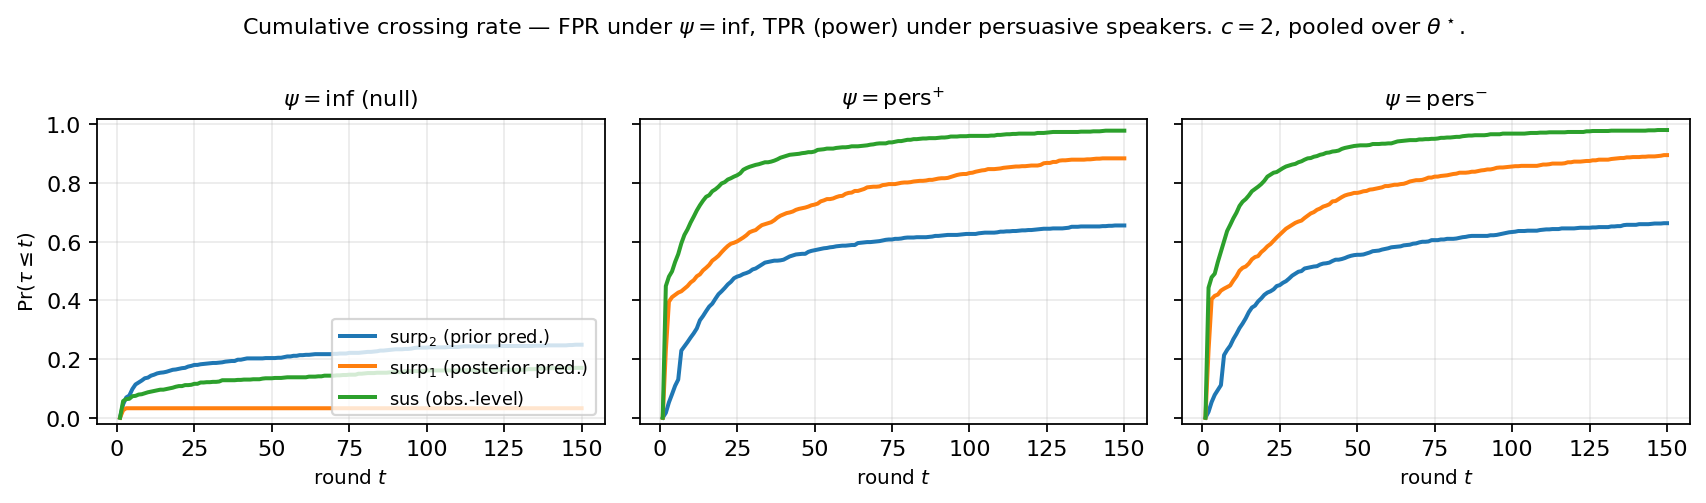
\includegraphics[width=0.98\linewidth]{full_power_curve.png}
\caption{Cumulative crossing rate $\Pr(\tau\leq t)$ as a function of round
$t$, for each speaker type.  Left panel is the FPR (any crossing under the
null is a false alarm); the two right panels are detection power (TPR)
under persuasive speakers.  Curves are pooled over all nine $\theta^\star$
values.}
\end{figure}

\begin{figure}[H]
\centering
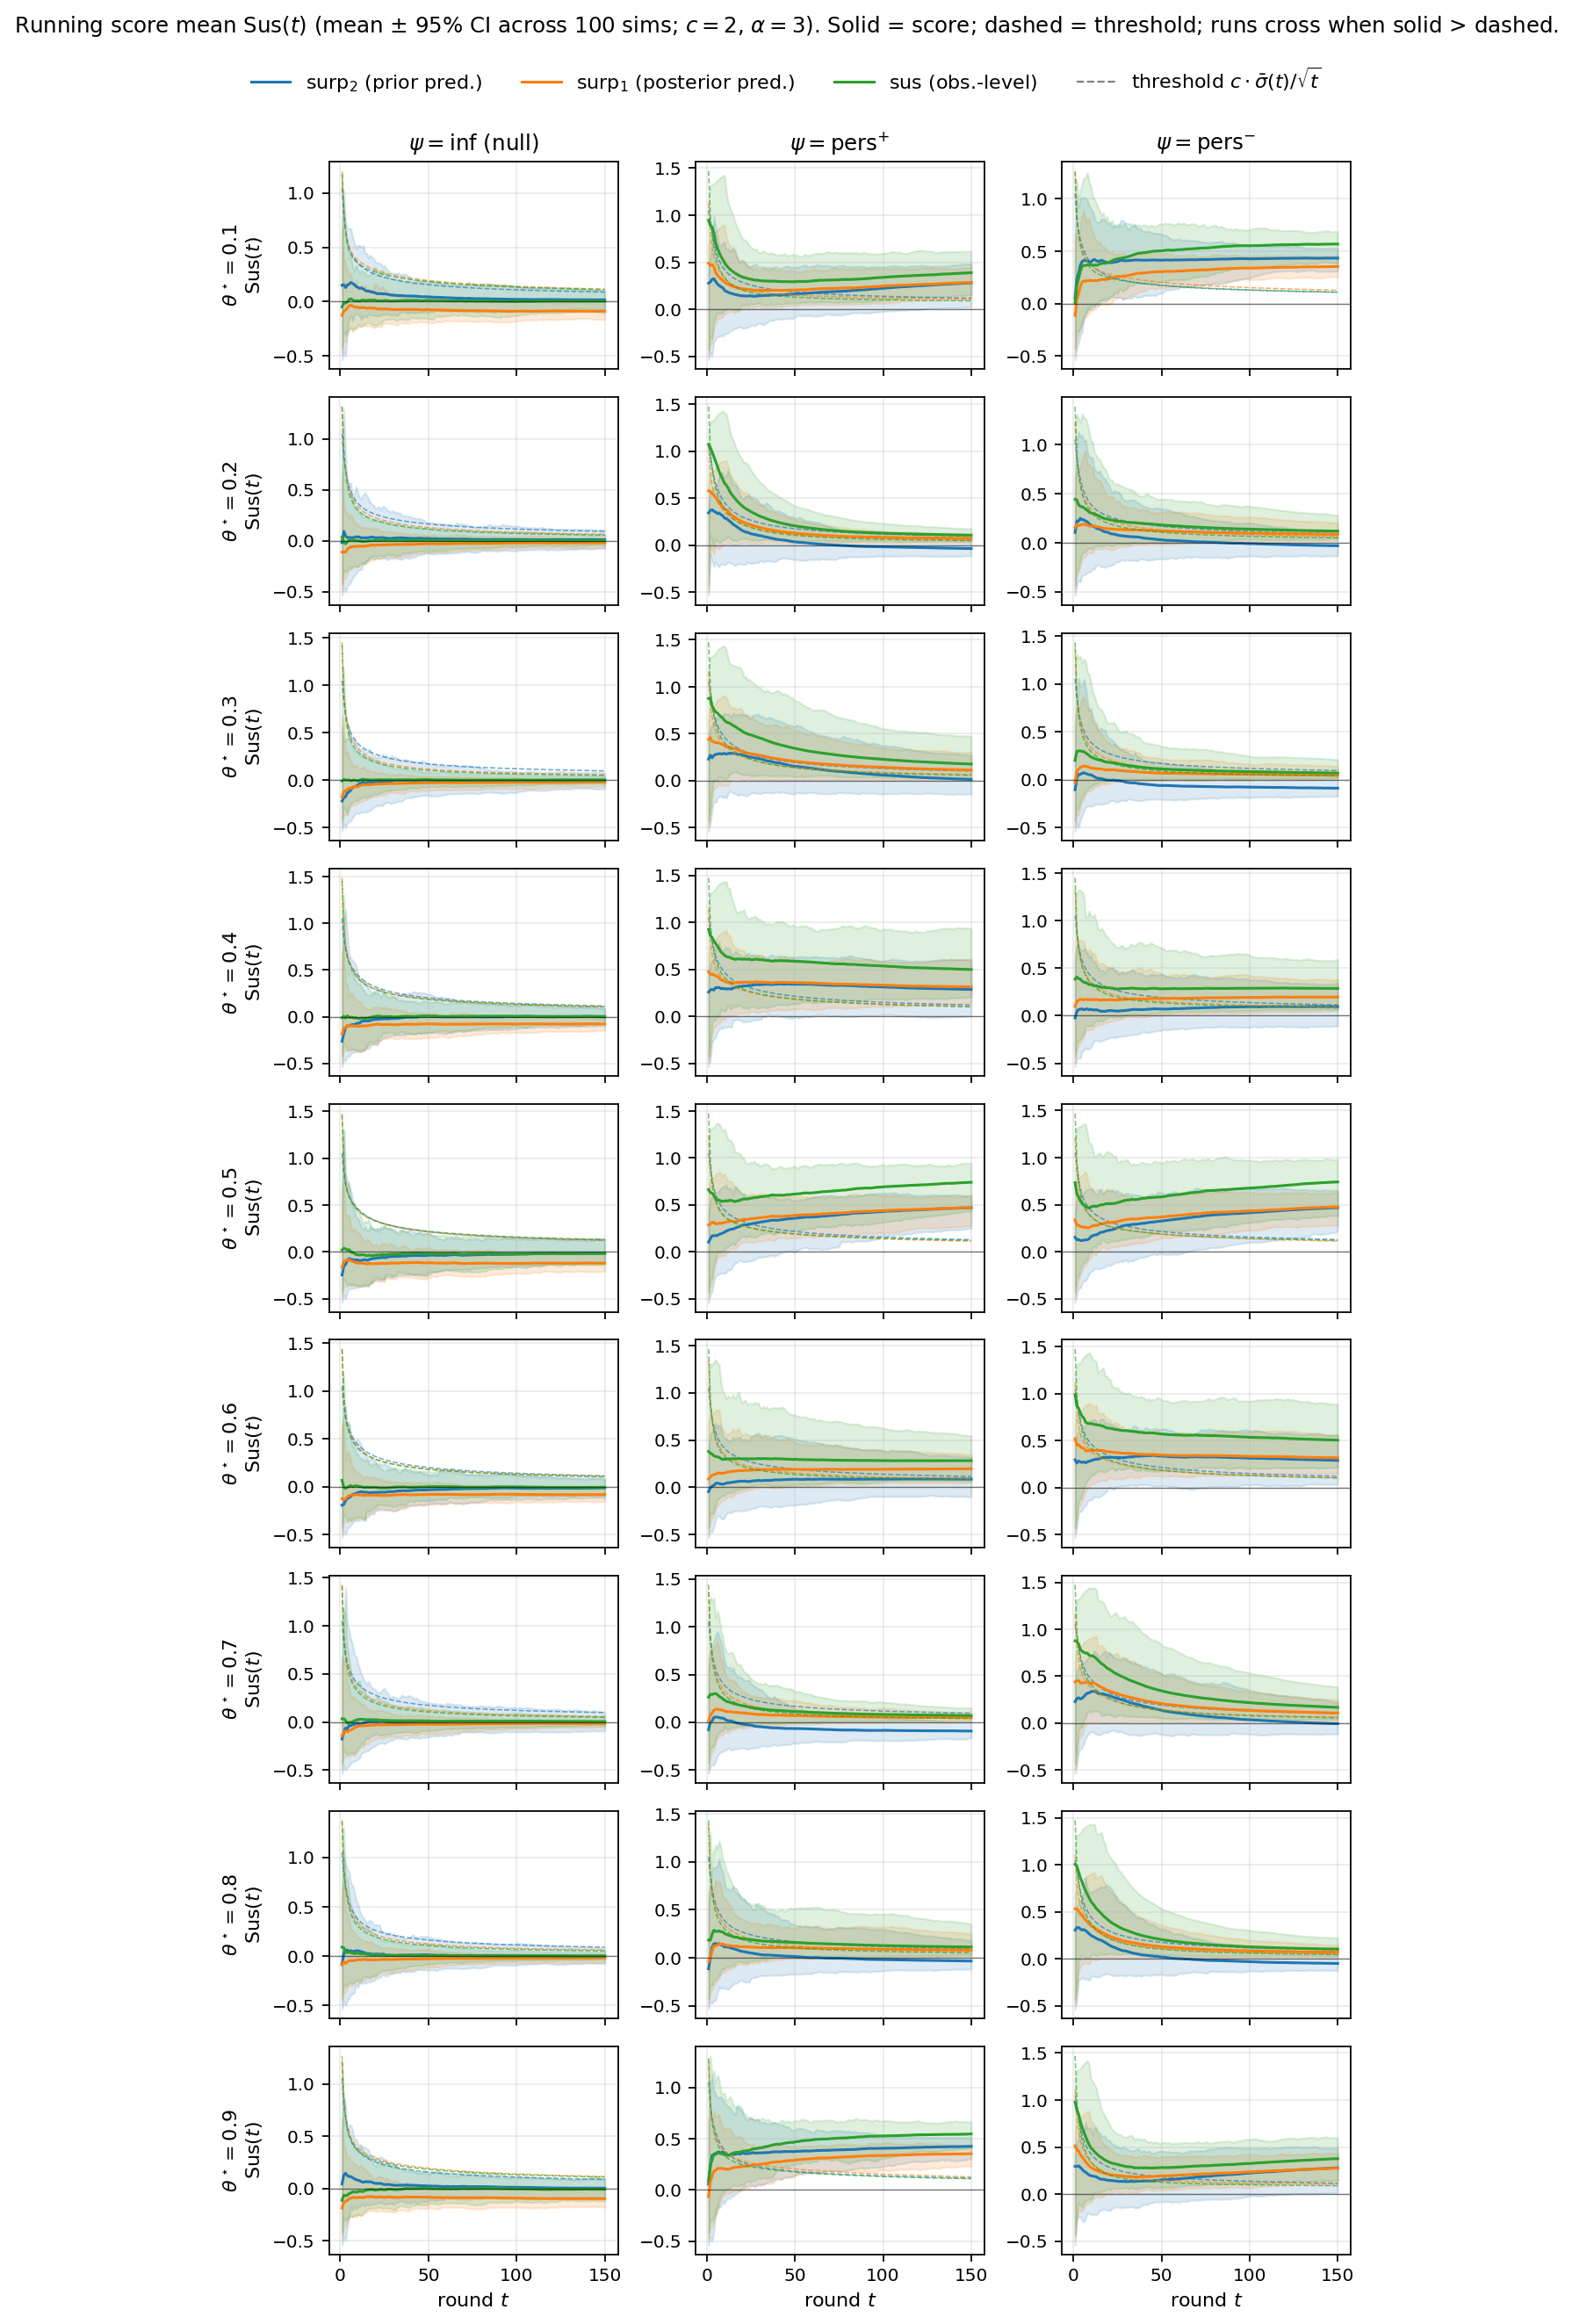
\includegraphics[width=0.98\linewidth]{full_trajectories.png}
\caption{Running score mean $\Sus(t)$ by $(\psi,\theta^\star)$.  Solid
lines are across-sim means with a 95\,\% band; dashed lines are the
corresponding mean thresholds $c\,\bar\sigma(t)/\sqrt{t}$.  A run crosses
when its solid line passes above its dashed line.}
\end{figure}

\begin{figure}[H]
\centering
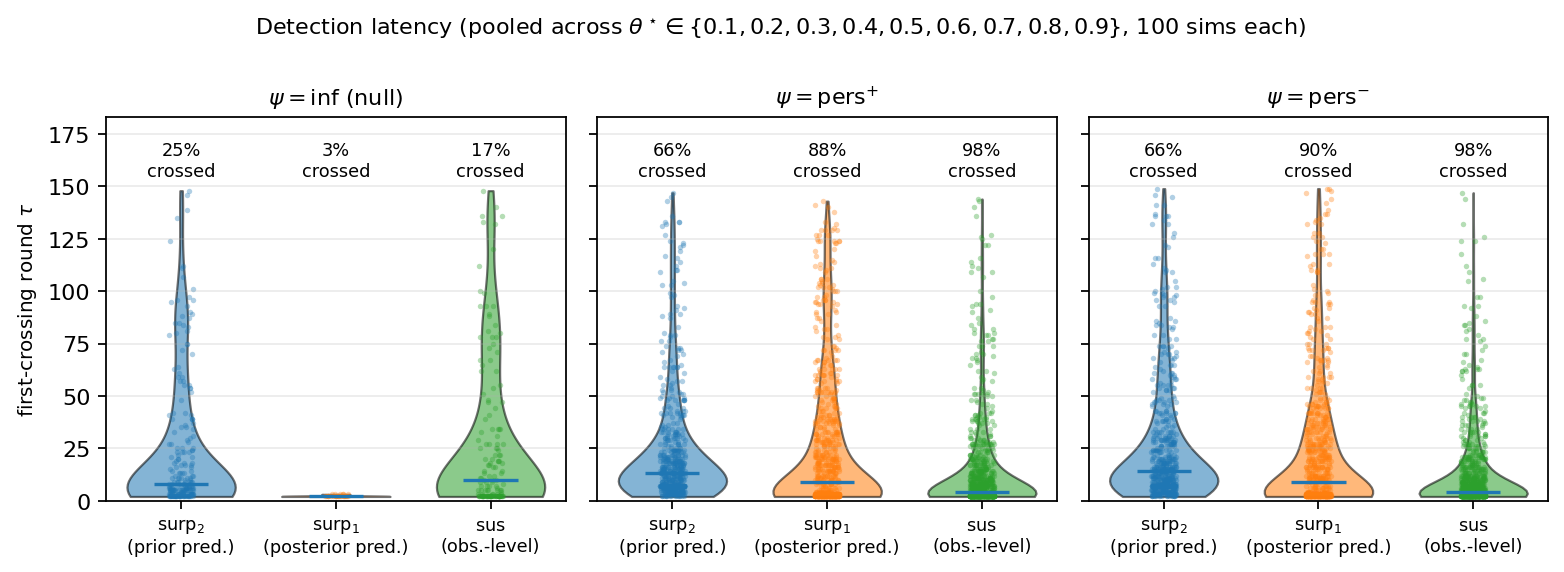
\includegraphics[width=0.98\linewidth]{full_latency.png}
\caption{Distribution of first-crossing round $\tau$ pooled over
$\theta^\star$.  Violins use only simulations that crossed; the percentage
above each violin is the fraction of simulations that ever crossed within
150 rounds.  Points are jittered individual $\tau$ values.}
\end{figure}

\begin{figure}[H]
\centering
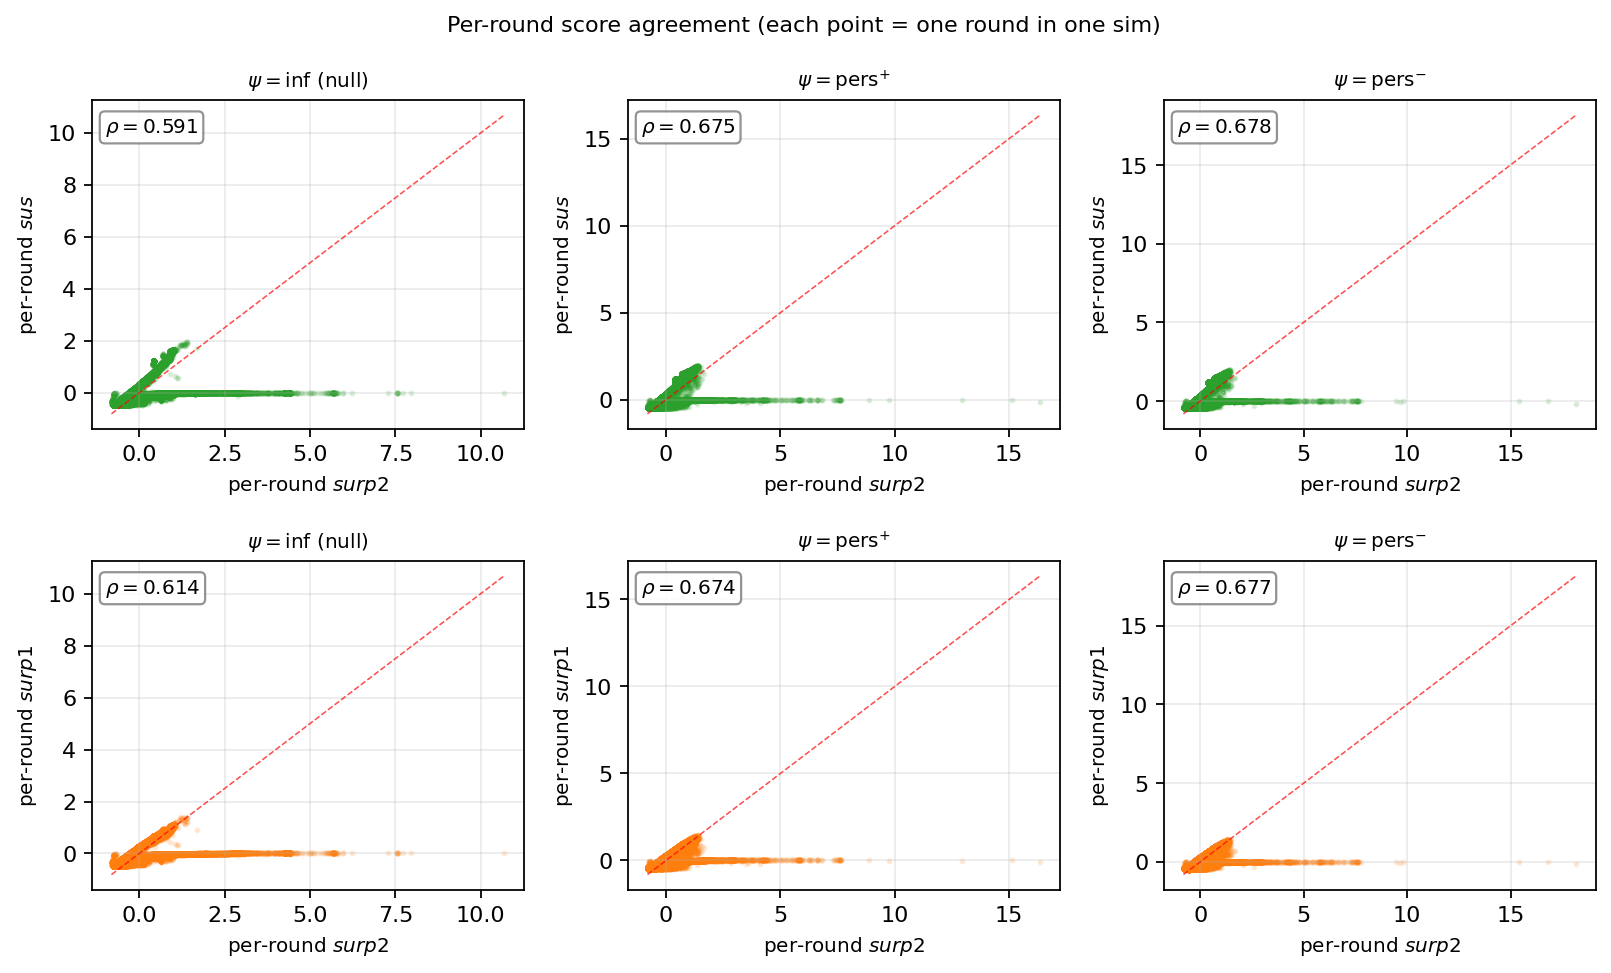
\includegraphics[width=0.98\linewidth]{full_correlation.png}
\caption{Per-round score agreement.  Each point is a single round in a
single simulation; colour encodes the score on the $y$-axis.  The red
dashed line is $y=x$.  Pearson correlations are shown inset.}
\end{figure}

\section{Brief analysis}

\paragraph{Headline.} \texttt{sus} dominates on raw power (TPR$=98.0$\,\%, vs.\ $\texttt{surp1}$:\,89.0\,\%, $\texttt{surp2}$:\,65.9\,\%), while \texttt{surp1} attains the lowest false-alarm rate (FPR$=3.2$\,\% vs.\ $\texttt{sus}$:\,17.0\,\%, $\texttt{surp2}$:\,24.9\,\%).  By the marginal TPR$-$FPR gap, \texttt{surp1} wins (85.8\,\%); by raw TPR, \texttt{sus} wins.  The right choice depends on whether one prioritises calibration or sensitivity -- both posterior-based scores ($\texttt{surp1}$, $\texttt{sus}$) clearly dominate the prior-predictive baseline $\texttt{surp2}$ on every aggregate metric.  \paragraph{Hardest case.} The hardest persuasive condition is $(\psi{=}\pers^{+},\,\theta^\star{=}0.7)$: pooled detection across scores is only 52\,\% (\texttt{surp2}: 18\,\%, \texttt{surp1}: 49\,\%, \texttt{sus}: 88\,\%).  This is the regime where the speaker's persuasive bias aligns with the prior over $\theta$, so the utterance distribution under the persuasive speaker is hardest to distinguish from the informative one; only $\texttt{sus}$ remains well above chance.  \paragraph{Score correspondence.} The per-round scatter shows $\texttt{sus}$ and $\texttt{surp2}$ are strongly correlated but $\texttt{sus}$ compresses large-surprise tails and shifts the distribution downward -- exactly the behaviour predicted by the $-\KL\bigl(L_1(\cdot\mid u)\,\|\,L_1(\cdot)\bigr)$ correction in the algebraic identity, which subtracts more from $\surp_2$ precisely when the heard utterance is highly diagnostic of $O$.  Empirically this is what makes $\texttt{sus}$ both more powerful on persuasive speakers \emph{and} less prone to over-reacting to single tail utterances under the null.

\end{document}
